\providecommand{\main}{../..}
\documentclass[\main/thesis.tex]{subfiles}
\begin{document}

\section{Incrementing a Numeral}\label{increment}

Given a numeral \lstinline|xs| of \lstinline|Numeral b d o|
and a proof of \lstinline|¬ (Maximum xs)|,
with functions and theorems constructed in the last section, we can:

\begin{itemize}
    \item Find the next numeral of \lstinline|xs| using \lstinline|next-numeral|.
    \item Know that the next numeral will be greater than \lstinline|xs|
        by \lstinline|next-numeral-is-greater|.
    \item Know that the next numeral will be the least numeral that is greater
        than \lstinline|xs| by \lstinline|next-numeral-is-immediate|.
\end{itemize}

However, none of the theorems above guarantees that the next numeral will be the
\textbf{successor} of \lstinline|xs|, i.e., the next numeral and \lstinline|xs|
differs by only $ 1 $.
For example, we have seen from the previous section that numerals of
\lstinline|GappedEndpoint| of systems of \lstinline|Proper| have no successors.

\begin{figure}[H]
    \centering
    \begin{adjustbox}{max width=\textwidth}
        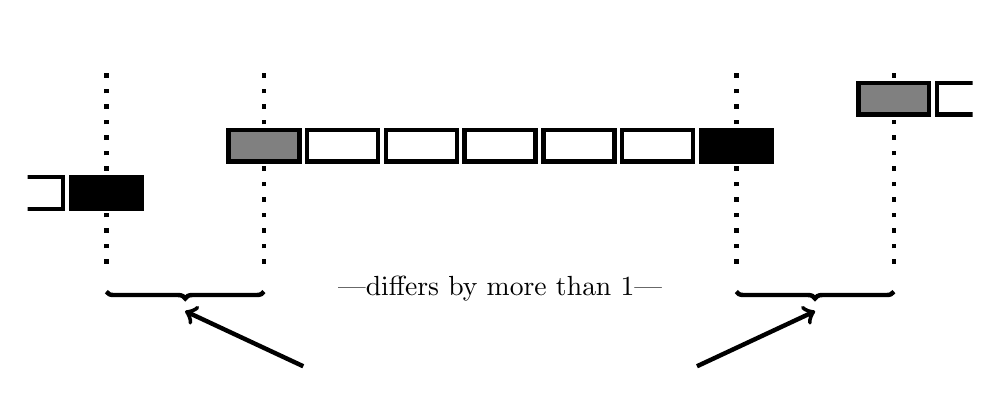
\begin{tikzpicture}
            % the frame
            \path[clip] (5.5, -3) rectangle (17.5, 1.5);


            % ticks
            \draw[ultra thick, loosely dotted] (6.5,-1.5) -- (6.5,1);
            \draw[ultra thick, loosely dotted] (8.5,-1.5) -- (8.5,1);
            \draw[ultra thick, loosely dotted] (14.5,-1.5) -- (14.5,1);
            \draw[ultra thick, loosely dotted] (16.5,-1.5) -- (16.5,1);

            \draw[ultra thick, decoration={brace,mirror,raise=10},decorate]
                (6.5,-1.5) -- (8.5,-1.5);
            \draw[ultra thick, decoration={brace,mirror,raise=10},decorate]
                (14.5,-1.5) -- (16.5,-1.5);
            \node[below=1] at (11.5, -1.5) {\lstinline|differs by more than 1|};

            % the body
            \foreach \i in {0,...,2} {
                \draw[ultra thick, fill=gray] ({\i*8+0.05}, {\i*0.6-0.8}) rectangle ({\i*8+0.95}, {\i*0.6-0.4});
                \foreach \j in {1,...,5} {
                    \draw[ultra thick] ({\i*8+\j+0.05}, {\i*0.6-0.8}) rectangle ({\i*8+\j+0.95}, {\i*0.6-0.4});
                };
                \draw[ultra thick, fill=black] ({\i*8+6.05}, {\i*0.6-0.8}) rectangle ({\i*8+6.95}, {\i*0.6-0.4});
            };

            \coordinate (A) at (7.5, -2.1);
            \coordinate (B) at (9, -2.8);
            \coordinate (C) at (15.5, -2.1);
            \coordinate (D) at (14, -2.8);

            \path[->, ultra thick] (B) edge node {} (A);
            \path[->, ultra thick] (D) edge node {} (C);

        \end{tikzpicture}
    \end{adjustbox}
\caption{The cause of gaps}
\label{figure:26}
\end{figure}

Suppose we are to define a function called \lstinline|increment| that returns
the successor of a given numeral.
For those numerals that are eligible for increment,
we can simply compute them with \lstinline|next-numeral|;
and for those that are not eligible, we need a predicate for discriminating them.

\subsection{\lstinline|Incrementable|}

Similar to the definition of \lstinline|Bounded|, we define the predicate
\lstinline|Incrementable| as an existential proposition.
To prove that a numeral \lstinline|xs| is \lstinline|Incrementable|,
one is obliged to present the successor \textit{and} a proof to justify it.

\begin{lstlisting}[basicstyle=\ttfamily\scriptsize]
Incrementable : ∀ {b d o} → (xs : Numeral b d o) → Set
Incrementable {b} {d} {o} xs = Σ[ xs' ∈ Numeral b d o ] ⟦ xs' ⟧ ≡ suc ⟦ xs ⟧
\end{lstlisting}

We can then develop lemmata and theorems about \lstinline|Incrementable|.

\subsubsection{Maximum Numerals}

If a numeral is a maximum, then there is no such a thing as the next numeral,
much less a successor.

\begin{lstlisting}
Maximum⇒¬Incrementable : ∀ {b d o}
    → (xs : Numeral b d o)
    → (max : Maximum xs)
    → ¬ (Incrementable xs)
Maximum⇒¬Incrementable xs max (incremented , claim)
    = contradiction
        (max incremented)
        (>⇒≰ (m≡1+n⇒m>n claim))
%
\end{lstlisting}
where \lstinline|incremented| is the claimed successor
and \lstinline|claim : ⟦ incremented ⟧ ≡ suc ⟦ xs ⟧|.
This is proven by contradicting these two propositions:

\begin{itemize}
    \item \lstinline|max incremented : ⟦ xs ⟧ ≥ ⟦ incremented ⟧|
    \item \lstinline|>⇒≰ (m≡1+n⇒m>n claim) : ⟦ xs ⟧ ≰ ⟦ incremented ⟧|
\end{itemize}

\subsubsection{Numerals in Intervals}

Numerals that are located in intervals of digit lines have successors.

\begin{figure}[H]
    \centering
        \begin{adjustbox}{max width=\textwidth}
        \begin{tikzpicture}
            % the frame
            \path[clip] (5.5, -1.5) rectangle (17.5, 1.5);

            % the body
            \foreach \i in {0,...,2} {
                \foreach \j in {0,...,5} {
                    \draw[ultra thick, fill=black] ({\i*8+\j+0.05}, {\i*0.6-0.8}) rectangle ({\i*8+\j+0.95}, {\i*0.6-0.4});
                };
                \draw[ultra thick, fill=gray] ({\i*8+6.05}, {\i*0.6-0.8}) rectangle ({\i*8+6.95}, {\i*0.6-0.4});
            };

            \foreach \i in {5,...,6} {
                \coordinate (\i) at ({\i + 0.5}, -0.9);
            };
            \foreach \i in {8,...,15} {
                \coordinate (\i) at ({\i + 0.5}, -0.3);
            };
            \foreach \i in {16,...,17} {
                \coordinate (\i) at ({\i + 0.5}, 0.3);
            };

            \foreach \i in {5,...,5} {
                \pgfmathsetmacro{\j}{\i + 1}
                \path[->, ultra thick] (\i) edge[bend right=60] node {} ($ (\j) + (-0.1, 0) $);
            };
            \foreach \i in {8,...,13} {
                \pgfmathsetmacro{\j}{\i + 1}
                \path[->, ultra thick] (\i) edge[bend right=60] node {} ($ (\j) + (-0.1, 0) $);
            };
            \foreach \i in {16,...,16} {
                \pgfmathsetmacro{\j}{\i + 1}
                \path[->, ultra thick] (\i) edge[bend right=60] node {} ($ (\j) + (-0.1, 0) $);
            };

        \end{tikzpicture}
    \end{adjustbox}
\caption{The case of intervals}
\label{figure:27}
\end{figure}

We invoke \lstinline|next-numeral-Proper-Interval-lemma| to establish the
successor relation between the given numeral and the next numeral.


\begin{lstlisting}[basicstyle=\ttfamily\scriptsize]
Interval⇒Incrementable : ∀ {b d o}
    → (xs : Numeral (suc b) (suc d) o)
    → (¬greatest : ¬ (Greatest (lsd xs)))
    → (proper : 2 ≤ suc (d + o))
    → Incrementable xs
Interval⇒Incrementable {b} {d} {o} xs ¬greatest proper
    = (next-numeral-Proper xs proper) , (begin
            ⟦ next-numeral-Proper xs proper ⟧
        ≡⟨ cong ⟦_⟧ (next-numeral-Proper-refine xs proper
            (Interval b d o ¬greatest))
        ⟩
            ⟦ next-numeral-Proper-Interval xs ¬greatest proper ⟧
        ≡⟨ next-numeral-Proper-Interval-lemma xs ¬greatest proper ⟩
            suc ⟦ xs ⟧
        ∎)
\end{lstlisting}

\subsubsection{Numerals at Gapped Endpoints}

Numerals that are located at gapped endpoints do not have successors.

\begin{figure}[H]
    \centering
    \begin{adjustbox}{max width=\textwidth}
        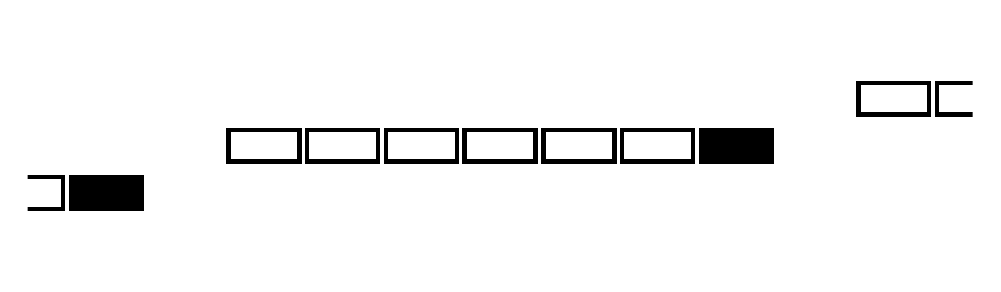
\begin{tikzpicture}
            % the frame
            \path[clip] (5.5, -1.5) rectangle (17.5, 1.5);

            % the body
            \foreach \i in {0,...,2} {
                \foreach \j in {0,...,5} {
                    \draw[ultra thick] ({\i*8+\j+0.05}, {\i*0.6-0.8}) rectangle ({\i*8+\j+0.95}, {\i*0.6-0.4});
                };
                \draw[ultra thick, fill=black] ({\i*8+6.05}, {\i*0.6-0.8}) rectangle ({\i*8+6.95}, {\i*0.6-0.4});
            };
        \end{tikzpicture}
    \end{adjustbox}
\caption{The case of gapped endpoints}
\label{figure:27}
\end{figure}

\begin{lstlisting}[basicstyle=\ttfamily\scriptsize]
GappedEndpoint⇒¬Incrementable : ∀ {b d o}
    → (xs : Numeral (suc b) (suc d) o)
    → (greatest : Greatest (lsd xs))
    → (proper : 2 ≤ suc (d + o))
    → (gapped : Gapped xs proper)
    → ¬ (Incrementable xs)
GappedEndpoint⇒¬Incrementable xs greatest proper gapped (incremented , claim)
    = contradiction ⟦next⟧>⟦incremented⟧ ⟦next⟧≯⟦incremented⟧
\end{lstlisting}

This is proven by contradicting two propositions as well.

First, we show that the next numeral is greater than the claimed successor
by rephrasing the lemma \lstinline|next-numeral-Proper-GappedEndpoint-lemma|.
As a side note, \lstinline|next-numeral-Proper| delegates tasks to other helper
functions. \lstinline|next-numeral-Proper-refine| is here to narrow the term
computed by \lstinline|next-numeral-Proper| down to
\lstinline|next-numeral-Proper-GappedEndpoint|
by providing evidence that the computation is delegated that way.

\begin{lstlisting}[basicstyle=\ttfamily\scriptsize]
⟦next⟧>⟦incremented⟧ : ⟦ next-numeral-Proper xs proper ⟧ > ⟦ incremented ⟧
⟦next⟧>⟦incremented⟧ =
    start
        suc ⟦ incremented ⟧
    ≈⟨ cong suc claim ⟩
        suc (suc ⟦ xs ⟧)
    ≤⟨ next-numeral-Proper-GappedEndpoint-lemma xs greatest proper gapped ⟩
        ⟦ next-numeral-Proper-GappedEndpoint xs proper gapped ⟧
    ≈⟨ cong ⟦_⟧ (sym (next-numeral-Proper-refine
        xs proper (GappedEndpoint b d o greatest gapped)))
    ⟩
        ⟦ next-numeral-Proper xs proper ⟧
    □
\end{lstlisting}

However, the next numeral should only be greater than the given numeral
\lstinline|xs| and nothing else.

\begin{lstlisting}[basicstyle=\ttfamily\scriptsize]
⟦next⟧≯⟦incremented⟧ : ⟦ next-numeral-Proper xs proper ⟧ ≯ ⟦ incremented ⟧
⟦next⟧≯⟦incremented⟧ = ≤⇒≯ (next-numeral-is-immediate-Proper
    xs incremented proper (m≡1+n⇒m>n claim))
\end{lstlisting}

\subsubsection{Numerals at Ungapped Endpoints}

Numerals that are located at ungapped endpoints also possess successors.

\begin{figure}[H]
    \centering
    \begin{adjustbox}{max width=\textwidth}
        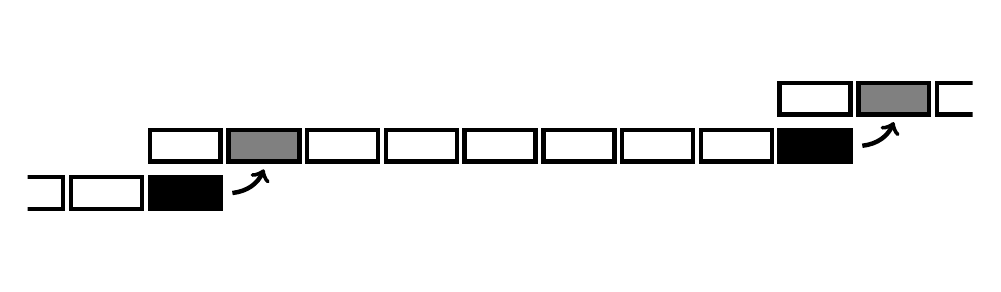
\begin{tikzpicture}
            % the frame
            \path[clip] (6.5, -1.5) rectangle (18.5, 1.5);

            % the body
            \foreach \i in {0,...,2} {
                \draw[ultra thick] ({\i*8+0.05}, {\i*0.6-0.8}) rectangle ({\i*8+0.95}, {\i*0.6-0.4});
                \draw[ultra thick, fill=gray] ({\i*8+1.05}, {\i*0.6-0.8}) rectangle ({\i*8+1.95}, {\i*0.6-0.4});
                \foreach \j in {2,...,7} {
                    \draw[ultra thick] ({\i*8+\j+0.05}, {\i*0.6-0.8}) rectangle ({\i*8+\j+0.95}, {\i*0.6-0.4});
                };
                \draw[ultra thick, fill=black] ({\i*8+8.05}, {\i*0.6-0.8}) rectangle ({\i*8+8.95}, {\i*0.6-0.4});
            };
            % arrows
            \coordinate (A) at (9.1, -0.6);
            \coordinate (B) at (9.5, -0.3);
            \coordinate (C) at (17.1, 0);
            \coordinate (D) at (17.5, 0.3);

            \path[->, ultra thick] (A) edge[bend right] node {} (B);
            \path[->, ultra thick] (C) edge[bend right] node {} (D);
        \end{tikzpicture}
    \end{adjustbox}
\caption{The case of ungapped endpoints}
\label{figure:28}
\end{figure}


Similar to the case of \lstinline|Interval|, the key to the proof lies in the
help of \lstinline|next-numeral-Proper-UngappedEndpoint-lemma|.

\begin{lstlisting}[basicstyle=\ttfamily\scriptsize]
UngappedEndpoint⇒Incrementable : ∀ {b d o}
    → (xs : Numeral (suc b) (suc d) o)
    → (greatest : Greatest (lsd xs))
    → (proper : 2 ≤ suc (d + o))
    → (¬gapped : ¬ (Gapped xs proper))
    → Incrementable xs
UngappedEndpoint⇒Incrementable {b} {d} {o} xs greatest proper ¬gapped
    = (next-numeral-Proper xs proper) , (begin
          ⟦ next-numeral-Proper xs proper ⟧
      ≡⟨ cong ⟦_⟧ (next-numeral-Proper-refine xs proper
          (UngappedEndpoint b d o greatest ¬gapped)) ⟩
          ⟦ next-numeral-Proper-UngappedEndpoint xs greatest proper ¬gapped ⟧
      ≡⟨ next-numeral-Proper-UngappedEndpoint-lemma xs greatest proper ¬gapped ⟩
          suc ⟦ xs ⟧
      ∎)
\end{lstlisting}

\subsection{Deciding Incrementable Numerals}

With all of the lemmata above, we can finish the most difficult part
of the decider.

\begin{lstlisting}[basicstyle=\ttfamily\scriptsize]
Incrementable?-Proper : ∀ {b d o}
    → (xs : Numeral (suc b) (suc d) o)
    → (proper : 2 ≤ suc (d + o))
    → Dec (Incrementable xs)
Incrementable?-Proper xs proper with nextView xs proper
Incrementable?-Proper xs proper | Interval b d o ¬greatest
    = yes (Interval⇒Incrementable xs ¬greatest proper)
Incrementable?-Proper xs proper | GappedEndpoint b d o greatest gapped
    = no (GappedEndpoint⇒¬Incrementable xs greatest proper gapped)
Incrementable?-Proper xs proper | UngappedEndpoint b d o greatest ¬gapped
    = yes (UngappedEndpoint⇒Incrementable xs greatest proper ¬gapped)
\end{lstlisting}

We can determine if numerals of other categories are incrementable as well.

\begin{lstlisting}
Incrementable? : ∀ {b d o}
    → (xs : Numeral b d o)
    → Dec (Incrementable xs)
Incrementable? xs with Maximum? xs
Incrementable? xs | yes max = no (Maximum⇒¬Incrementable xs max)
Incrementable? {b} {d} {o} xs | no ¬max with numView b d o
Incrementable? xs | no ¬max | NullBase d o
    = yes ((next-numeral-NullBase xs ¬max) ,
        (next-numeral-NullBase-lemma xs ¬max))
Incrementable? xs | no ¬max | NoDigits b o
    = yes (NoDigits-explode xs)
Incrementable? xs | no ¬max | AllZeros b
    = no (contradiction (Maximum-AllZeros xs) ¬max)
Incrementable? xs | no ¬max | Proper b d o proper
    = Incrementable?-Proper xs proper
\end{lstlisting}

The table below sums up whether a non-maximum numeral can be incremented in
systems of each category.

\begin{table}[H]
    \centering
    \begin{adjustbox}{max width=\textwidth}
    \begin{tabular}{|c|c|c|c|c|c|}
        \hline
        \multirow{2}{*}{\textbf{NullBase}} &
        \multirow{2}{*}{\textbf{NoDigits}} &
        \multirow{2}{*}{\textbf{AllZeros}} &
        \multicolumn{3}{c|}{\textbf{Proper}} \\
        \cline{4 - 6}
        & & & \textbf{Inteval} & \textbf{Gapped} & \textbf{Ungapped} \\
        \hline
        yes & yes & no & yes & no & yes \\
        \hline
    \end{tabular}
    \end{adjustbox}
\caption{Summary of whether a non-maximum numeral can be incremented in
systems of each category}
\label{table:12}
\end{table}


Note that the decision of making numerals of \lstinline{NoDigits} incrementable
is completely arbitrary as it will always hold vacuously.

\subsection{\lstinline|increment|}

We can actually do without the previous section about \lstinline|Incrementable?|
and still be able to define a function that increments numerals.
All we have to do is to ask the user to prove that the numeral he or she has
given is incrementable.
By doing so, the user is obliged to provide the actual successor,
and then we can steal it and pretend that we have found the successor.
How outrageous!

\begin{lstlisting}
increment : ∀ {b d o}
    → (xs : Numeral b d o)
    → (incr : Incrementable xs)
    → Numeral b d o
increment xs incr = proj₁ incr
\end{lstlisting}

Obviously this is not the desired implementation of \lstinline|increment|.
The reason why we construct \lstinline|Incrementable?| is that it not only
does the real work of computing successors for us (the credit also goes to \lstinline|next-numeral|)
but also explains why a numeral is incrementable (or not).

The decidability of \lstinline|Incrementable?| enables us to embed it in types.
To filter out numerals that are not eligible for increment, we use the same trick
as when implementing safe \lstinline|head| on lists.

\begin{lstlisting}
True : {P : Set} → Dec P → Set
True (yes _) = ⊤
True (no _) = ⊥
\end{lstlisting}

\lstinline|True| translates positive results of a decidable predicate to
\lstinline|⊤| and negative results to \lstinline|⊥|,
where as \lstinline|toWitness| reclaims the proof of the given proposition for us.

\begin{lstlisting}
toWitness : {P : Set} {Q : Dec P} → True Q → P
toWitness {Q = yes p} _  = p
toWitness {Q = no  _} ()
\end{lstlisting}

Finally, the true implementation of \lstinline|increment| is as follows:

\begin{lstlisting}
increment : ∀ {b d o}
    → (xs : Numeral b d o)
    → (incr : True (Incrementable? xs))
    → Numeral b d o
increment xs incr = proj₁ (toWitness incr)
\end{lstlisting}

\subsection{Properties of \lstinline|increment|}

\begin{lstlisting}
increment-next-numeral : ∀ {b d o}
    → (xs : Numeral b d o)
    → (¬max : ¬ (Maximum xs))
    → (incr : True (Incrementable? xs))
    → increment xs incr ≡ next-numeral xs ¬max
\end{lstlisting}

This property relates \lstinline|increment| with \lstinline|next-numeral|.
It may look trivial, however, the underlying implementation of \lstinline|increment|
does not actually involve \lstinline|next-numeral|, but helper functions like
\lstinline|next-numeral-Proper| and \lstinline|next-numeral-NullBase|.
We dispense with the proof of this property as it is comprised mostly of pattern
matching and seemly meaningless \lstinline|refl|s.
\end{document}
